\section{Pattern Matching with Typed Holes in Hazel}\label{sec:pattern-matching}

Let us now return to the problem of extending Hazel with pattern matching, placing particular emphasis on maintaining Hazel's maximal liveness invariant. Presently, all current systems with typed-holes only support holes in expressions or types, but notably, do not permit holes in binding constructs such as patterns. As a result, when editing a pattern - a necessarily incremental process - a user still faces meaningless editor states and thus gaps in editor services. To resolve this, we again turn to the approach outlined in \cite{DBLP:conf/snapl/OmarVHSGAH17}, extending our language to represent such intermediate pattern edit states as well-formed terms. 

Note that, for our purposes, patterns and expressions are quite similar: both are built up compositionally and are subject to typing restrictions. Correspondingly, we proceed by introducing two variants of \emph{pattern holes}. We include \emph{empty pattern holes} to indicate a missing sub-term of a pattern, and we include \emph{non-empty pattern holes} to act as a membrane around patterns that are ill-typed with regards to their location in a larger pattern. Syntactically, pattern holes indeed enable us to represent any pattern edit state without much difficulty, and they are fairly trivial to implement into our extension of Hazel. Semantically, however, the situation is much more subtle. 

At a high level, expression holes indicate \emph{unknown expressions} and pattern holes indicate \emph{unknown patterns}. Thus, whatever semantics we choose to give terms with holes, it must be sound with respect to all possible hole-fillings, and resultingly, we must reason conservatively about the contents of any particular hole. At the same time, we must strike a balance, limiting this conservativeness as much as possible in order to still provide viable static analysis and dynamic evaluation in cases where we can soundly do so without knowledge about the contents of any hole. For pattern matching, this balance manifests as stating that a match succeeds only if it succeeds in all possible (expression and pattern) hole-fillings. Likewise, a match fails only if it fails in all possible hole-fillings. However, as the astute reader will note, this leaves open a third possibility: some hole-fillings may result in a match succeeding while other hole-fillings result in the match failing - an expression may \emph{indeterminately} match a pattern. 

When we allow expression and pattern holes, we can then no longer determinately say whether an expression matches a given pattern. What was once a binary decision - either $e$ matches $p$ or $e$ does not match $p$ - is now a ternary decision: either $e$ must match $p$, $e$ must not match $p$, or $e$ indeterminately matches $p$ depending on how the various holes are filled. In turn, redundancy and exhaustiveness also become ternary decisions: a \li{match} expression may either be necessarily exhaustive, necessarily inexhaustive, or indeterminate, and likewise for redundancy. 

To more concretely present these subtleties, throughout the rest of this section we discuss a running example where the user edits an \li{odd_length} function, returning whether an input of type \li{[Int]} has an odd number of elements. We explore the full semantics of the \li{match} expression with live evaluation in \autoref{sec:live-eval}, then further explore exhaustiveness in \autoref{sec:exhaustiveness} and redundancy in \autoref{sec:redundancy}.

\subsection{Live Evaluation with Pattern Holes}\label{sec:live-eval}

As discussed, in order to support live evaluation with pattern holes, we must distinguish whether a given expression and pattern \emph{must} match, \emph{must not} match, or \emph{indeterminately} match. Let us consider how these different possibilities play out in \autoref{fig:evaluation-ex}, working through examples of a \li{match} expression with expression holes in the scrutinee and with pattern holes in the listed rules. The provided screenshots are from the Hazel implementation of our work.

\begin{figure}
	\centering
	% Capture tallest image in box 2
	\setbox2=\hbox{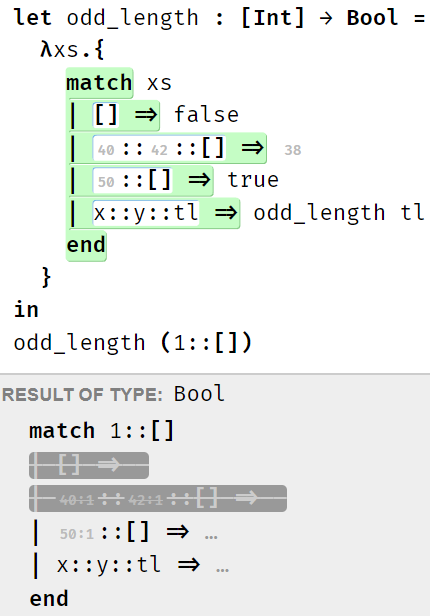
\includegraphics[scale=0.47]{imgs/pat_match_pat_holes.png}}%
	\subcaptionbox{Pattern matching with expression holes\label{fig:exp-hole}}{
		\raisebox{\dimexpr\ht2-\height}{
			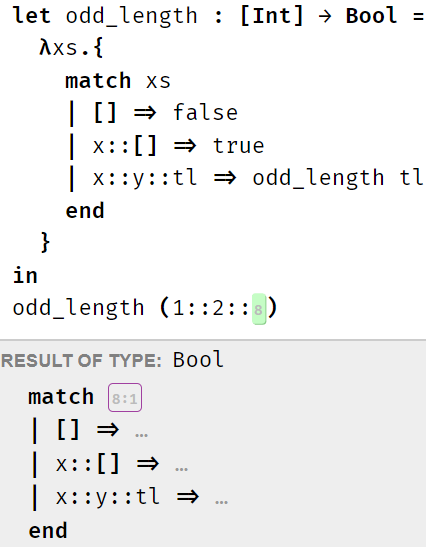
\includegraphics[scale=0.47,valign=t]{imgs/pat_match_exp_holes.png}
			\vphantom{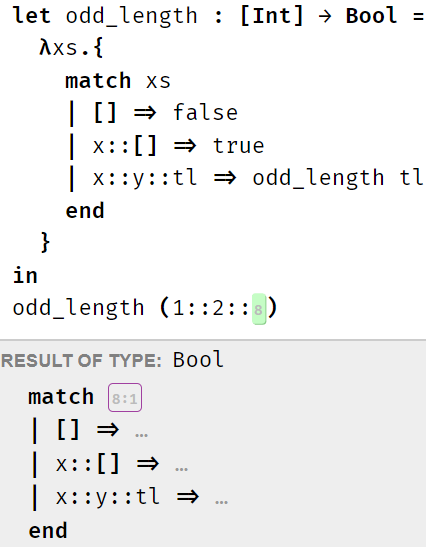
\includegraphics[scale=0.47,valign=t]{imgs/pat_match_exp_holes.png}}
		}
	}
	\hfil
	\subcaptionbox{Pattern matching with pattern holes\label{fig:pat-hole}}{
		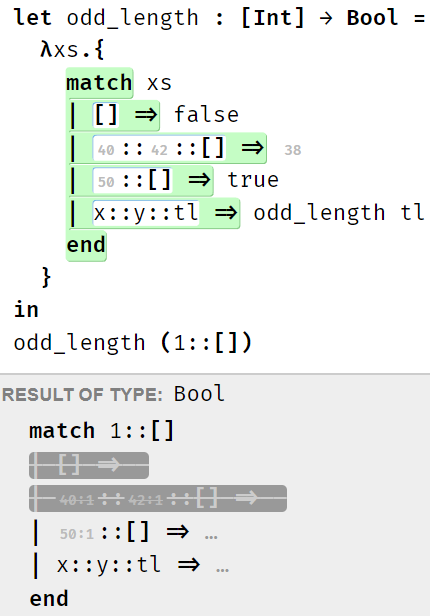
\includegraphics[scale=0.47,valign=t]{imgs/pat_match_pat_holes.png}
	}
	\caption{Live Evaluation with Expression and Pattern Holes}
	\label{fig:evaluation-ex}
\end{figure}


In \autoref{fig:exp-hole}, we apply the function \li{odd_length} to an argument that contains an expression hole with id \li{8}. Although the argument is indeterminate and cannot be fully-evaluated, per Hazel's live dynamic semantics, we still substitute it into the function body and continue as far as possible. Our argument then becomes the scrutinee of the \li{match} expression, and we proceed with pattern matching. Beginning with the first pattern, regardless of hole-filling, the outermost constructor of our scrutinee is the cons operator \li{::} rather than the empty list \li{[]}. Thus, our scrutinee must not match the first pattern \li{[]}, and we continue to the next rule. For the second pattern, regardless of hole-filling, our scrutinee always contains at least two elements while the pattern specifies only one element. Again then, our scrutinee must not match the second pattern, so evaluation moves to consider the third rule. Finally, as the scrutineee indeed always contains at least two elements, the third match succeeds in every hole-filling. Correspondingly, \li{x} is bound to \li{1}, \li{y} is bound to \li{2}, and \li{tl} is bound to the hole with id \li{8}. Evaluation then proceeds to the recursive call, and in this frame, our scrutinee becomes just an expression hole. Because we do not know whether the hole will be filled with an empty list or some other contents, we cannot determinately say whether it matches the first  pattern \li{[]}, hence evaluation must pause. We cannot proceed without further hole-filling, so the entire \li{match} expression becomes indeterminate, displayed as the final result at the bottom of the image. Note that the scrutinee in the final result is indeed just the expression hole with id \li{8}.

In \autoref{fig:pat-hole}, our argument no longer contains any expression holes, but indeterminacy still arises due to the pattern holes in the second and third rules of the \li{match} expression. Specifically, evaluation begins by analyzing the scrutinee against the first pattern, and as \li{1 :: []} is not the empty list, we determine it must not match the first pattern. Likewise, despite the presence of pattern holes, the second pattern may only be matched by a two element list, so our scrutinee must not match it, and we continue to the third pattern. The third pattern gives the most interesting case. It indeed specifies a list with a single element, but the head of the pattern is a  pattern hole with id \li{50}, indicating that the first element of the scrutinee must match some yet-unknown pattern. If hole \li{50} were filled with the integer pattern \li{1} or a variable \li{x}, then \li{1::[]} would match. However, for many other hole-fillings, e.g. the integer \li{2}, the match clearly fails. As a result, we can only state that \li{1::[]} indeterminately matches the third pattern, and evaluation must pause pending further hole-filling. Correspondingly, the entire \li{match} expression becomes indeterminate and is shown as the final result. By striking out the first two rules and displaying them in gray, we indicate to the user that evaluation has already proceeded past these cases.

\subsection{Exhaustiveness Checking with Pattern Holes}\label{sec:exhaustiveness}
With the dynamic semantics for live evaluation now clear, let us consider how to statically reason about this dynamic behavior through checks such as \emph{exhaustiveness analysis}. Recall that, in a language without holes, exhaustiveness requires that every expression of appropriate type matches at least one of the patterns in a \li{match} expression. When we introduce holes, however, exhaustiveness becomes more subtle, and we again must reason conservatively about all possible hole-fillings and thereby handle cases of indeterminacy.

\begin{figure}
	\centering
	% Capture tallest image in box 3
	\setbox3=\hbox{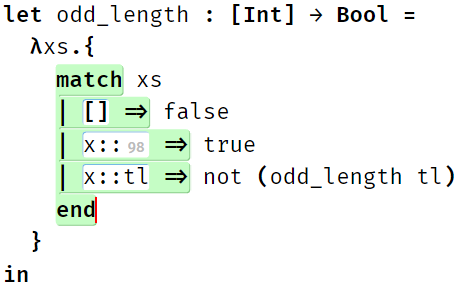
\includegraphics[scale=0.45]{imgs/exhaustive.png}}%
	\subcaptionbox{Indeterminately Exhaustive\label{fig:may-exhaustive}}{
		\raisebox{\dimexpr\ht3-\height}{
			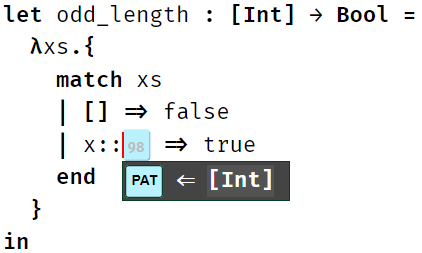
\includegraphics[scale=0.45,valign=t]{imgs/maybe_exhaustive.png}%
			\vphantom{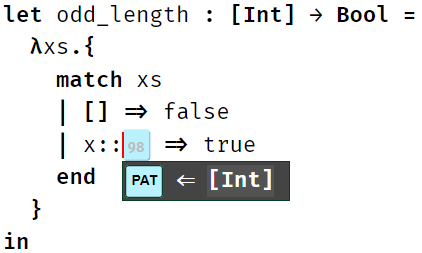
\includegraphics[scale=0.45,valign=t]{imgs/maybe_exhaustive.png}}
		}
	}
	\hfil
	\subcaptionbox{Necessarily Inexhaustive\label{fig:not-exhaustive}}{
		\raisebox{\dimexpr\ht3-\height}{
			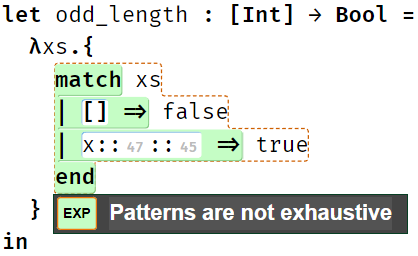
\includegraphics[scale=0.45,valign=t]{imgs/not_exhaustive.png}%
			\vphantom{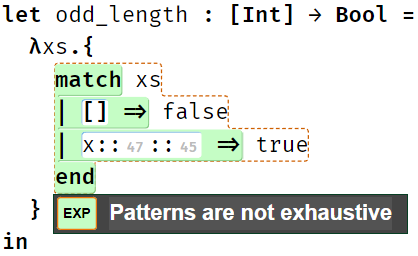
\includegraphics[scale=0.45,valign=t]{imgs/not_exhaustive.png}}
		}
	}
	\hfil
	\subcaptionbox{Necessarily Exhaustive\label{fig:must-exhaustive}}{
		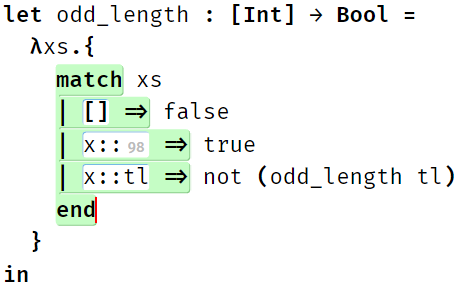
\includegraphics[scale=0.45,valign=t]{imgs/exhaustive.png}
	}
	\caption{Exhaustiveness Checking with Pattern Holes}
	\label{fig:exhaustiveness}
\end{figure}

Explicitly, assume the editor state is as in \autoref{fig:may-exhaustive}. The \li{match} expression contains two rules - the first with an empty list pattern \li{[]}, and the second with a cons cell pattern \li{::} containing a variable \li{x} at the head and a pattern hole at the tail. The cursor is placed over the pattern hole, and Hazel is able to infer the type of the pattern as \li{[Int]} from the surrounding context, presenting this information to the user. Should we consider such an expression to be exhaustive? If the user fills the pattern hole with a variable \li{xs}, then the \li{match} is indeed exhaustive: any empty list matches the first pattern, and any non-empty list matches the second pattern. However, if the user instead fills the hole with, say, \li{[]} or \li{y::tl}, then a list with three elements would fail to match any pattern. Thus, without further hole-filling, we can only soundly state that the \li{match} is \emph{indeterminately exhaustive}.

While we cannot guarantee exhaustiveness in \autoref{fig:may-exhaustive}, such indeterminacy does not necessarily reflect an error on the user's part. Instead, they may simply be in the middle of on-going editing, working towards what will soon become an exhaustive expression. To avoid distracting the user with unnecessary information in these cases, for Hazel, we choose not to alert the user of indeterminate exhaustiveness. Instead, we only report an error when, regardless of hole-fillings, the expression is always inexhaustive. We say such a \li{match} is \emph{necessarily inexhaustive}, and \autoref{fig:not-exhaustive} provides an illustrative example. The first given rule given only matches the empty list, and the second rule only possibly matches lists with at least two elements, with this holding regardless of the choice of hole-fillings. Thus, in any hole-filling, a one element list such as \li{1 :: []} will not match any of the given patterns, and correspondingly, we display an error to the user. Note that the entire \li{match} expression is also placed within a non-empty hole. This is necessary to prevent evaluation from getting "stuck" with no applicable rule when the scrutinee witnesses the inexhaustiveness.

Finally, even with the presence of pattern holes, there are still cases where we can in fact guarantee exhaustiveness. Considering \autoref{fig:must-exhaustive}, the first and third patterns together already cover all appropriately typed expressions. Thus, regardless of how the pattern hole in the second rule is filled, the \li{match} expression as a whole will always be exhaustive, i.e. it is \emph{necessarily exhaustive}. Note that we do not make a visual distinction between necessarily exhaustive and indeterminately exhaustive expressions, again because such information is more likely to be distracting than useful to the user. However, the semantic distinction is interesting to note, and it may be of use to future editor services designed around such holes. 

\subsection{Redundancy Checking with Pattern Holes}\label{sec:redundancy}
From a certain point of view, exhaustiveness checking guarantees a notion of \emph{sufficiency} - that the patterns in a \li{match} expression are sufficient to cover all possible values of the scrutinee's type. Redundancy checking, on the other hand, guarantees a notion of \emph{necessity} - that all the patterns in a \li{match} expressions are in fact required in that none is fully subsumed by other patterns earlier in the sequence. Explicitly, we say that a pattern $p$ in a \li{match} expression is redundant if, for every value $e$ of the scrutinee's type matching $p$, necessarily $e$ also matches some pattern $p^\prime$ preceding $p$ in the sequence of rules. Because a \li{match} expression considers rules one-by-one from the top down, a rule with a redundant pattern will be an unreachable code path. 

As the reader should now anticipate, including pattern holes again requires us to reason conservatively about all possible hole-fillings, thereby introducing indeterminacy into our analysis. That is, a pattern may be either \emph{necessarily redundant}, \emph{necessarily irredundant}, or \emph{indeterminately irredundant} due to the presence of expression or pattern holes. Similarly to how we handled exhaustiveness checking, we again only alert the user in cases where an error is guaranteed, i.e. when a rule is necessarily redundant.

\begin{figure}
	\centering
	\subcaptionbox{Necessarily Irredundant (first two patterns) + Indeterminately Irredundant (third pattern)\label{fig:may-redundant}}{
		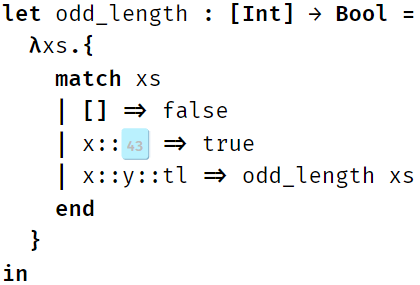
\includegraphics[scale=0.5,valign=t]{imgs/maybe_redundant.png}%
		\vphantom{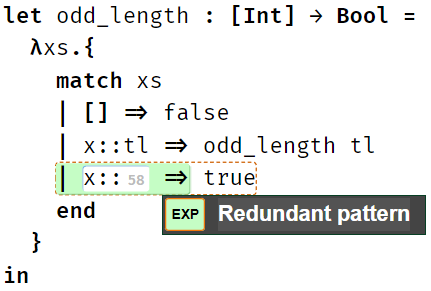
\includegraphics[scale=0.5,valign=t]{imgs/redundant.png}}
	} 
	\hfil
	\subcaptionbox{Necessarily Redundant (third pattern) \label{fig:must-redundant}}{
		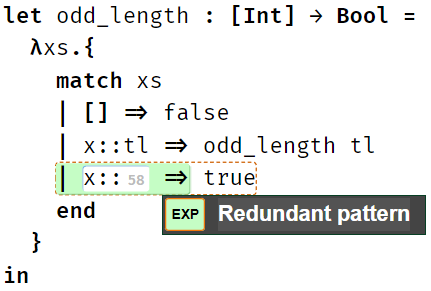
\includegraphics[scale=0.5,valign=t]{imgs/redundant.png}
	}%
	\caption{Redundancy Checking with Pattern Holes}
	\label{fig:redundancy}
\end{figure}

\autoref{fig:redundancy} concretely demonstrates all of these possibilities, continuing with our running example of an \li{odd_length} function. In the editor state in \autoref{fig:may-redundant}, there is a pattern hole in the second pattern. Depending on how this pattern hole is filled, the third pattern can be made either redundant or irredundant. Explicitly, if we filled the hole with the empty list \li{[]}, then the third pattern is the only one matching lists with more than one element, so it is irredundant. If instead we filled the hole with \li{y::tl}, then the second pattern is in fact the same as the third pattern, and obviously subsumes it. Thus, we can only soundly state that the third pattern is indeterminately irredundant.

For the second pattern itself, despite containing a pattern hole, we can still deem it necessarily irredundant. The only pattern preceding it is an empty list \li{[]}, while the second pattern only matches non-empty lists regardless of hole-filling. Thus, no hole-filling allows the second pattern to be made redundant by the first. Note that, vacuously, the first pattern is also necessarily irredundant - it cannot be subsumed by previous rules because there are no previous rules. Similarly, the first pattern of any \li{match} expression is necessarily irredundant, except in the case when the scrutinee's type has no values at all (e.g. is of \li{void} type). In this case, all rules are necessarily redundant.

Finally, the editor state in \autoref{fig:must-redundant} showcases a necessarily redundant pattern. Explicitly, regardless of the choice of hole-filling, the third pattern can only be matched by a non-empty list. However, the second pattern already matches all such non-empty lists. Thus, the third pattern is necessarily redundant, and correspondingly, we report an error to the user. Note that, in this particular case, the first two rules are already exhaustive, so any pattern we could possibly place in the third rule will be necessarily redundant. More generally, stating that a pattern $p$ is redundant is equivalent to stating that the preceding patterns exhaustively cover all values matching $p$. As we will explore in more detail in \autoref{sec:analyses}, this enables us to reduce the problem of redundancy checking to that of exhaustiveness checking.
